
\section{Modeling in Ptolemy}
\label{sec:modeling-ptolemy}

In this section, we present our work in Ptolemy that models the MAC layer of OpenWSN\footnote{Though the model in each figure is vector graphics, you can zoom in and read the details. We strongly suggest reader to open our Ptolemy model for details. These figures are mainly for illustration purpose.}.

\begin{figure}[t]
\centering
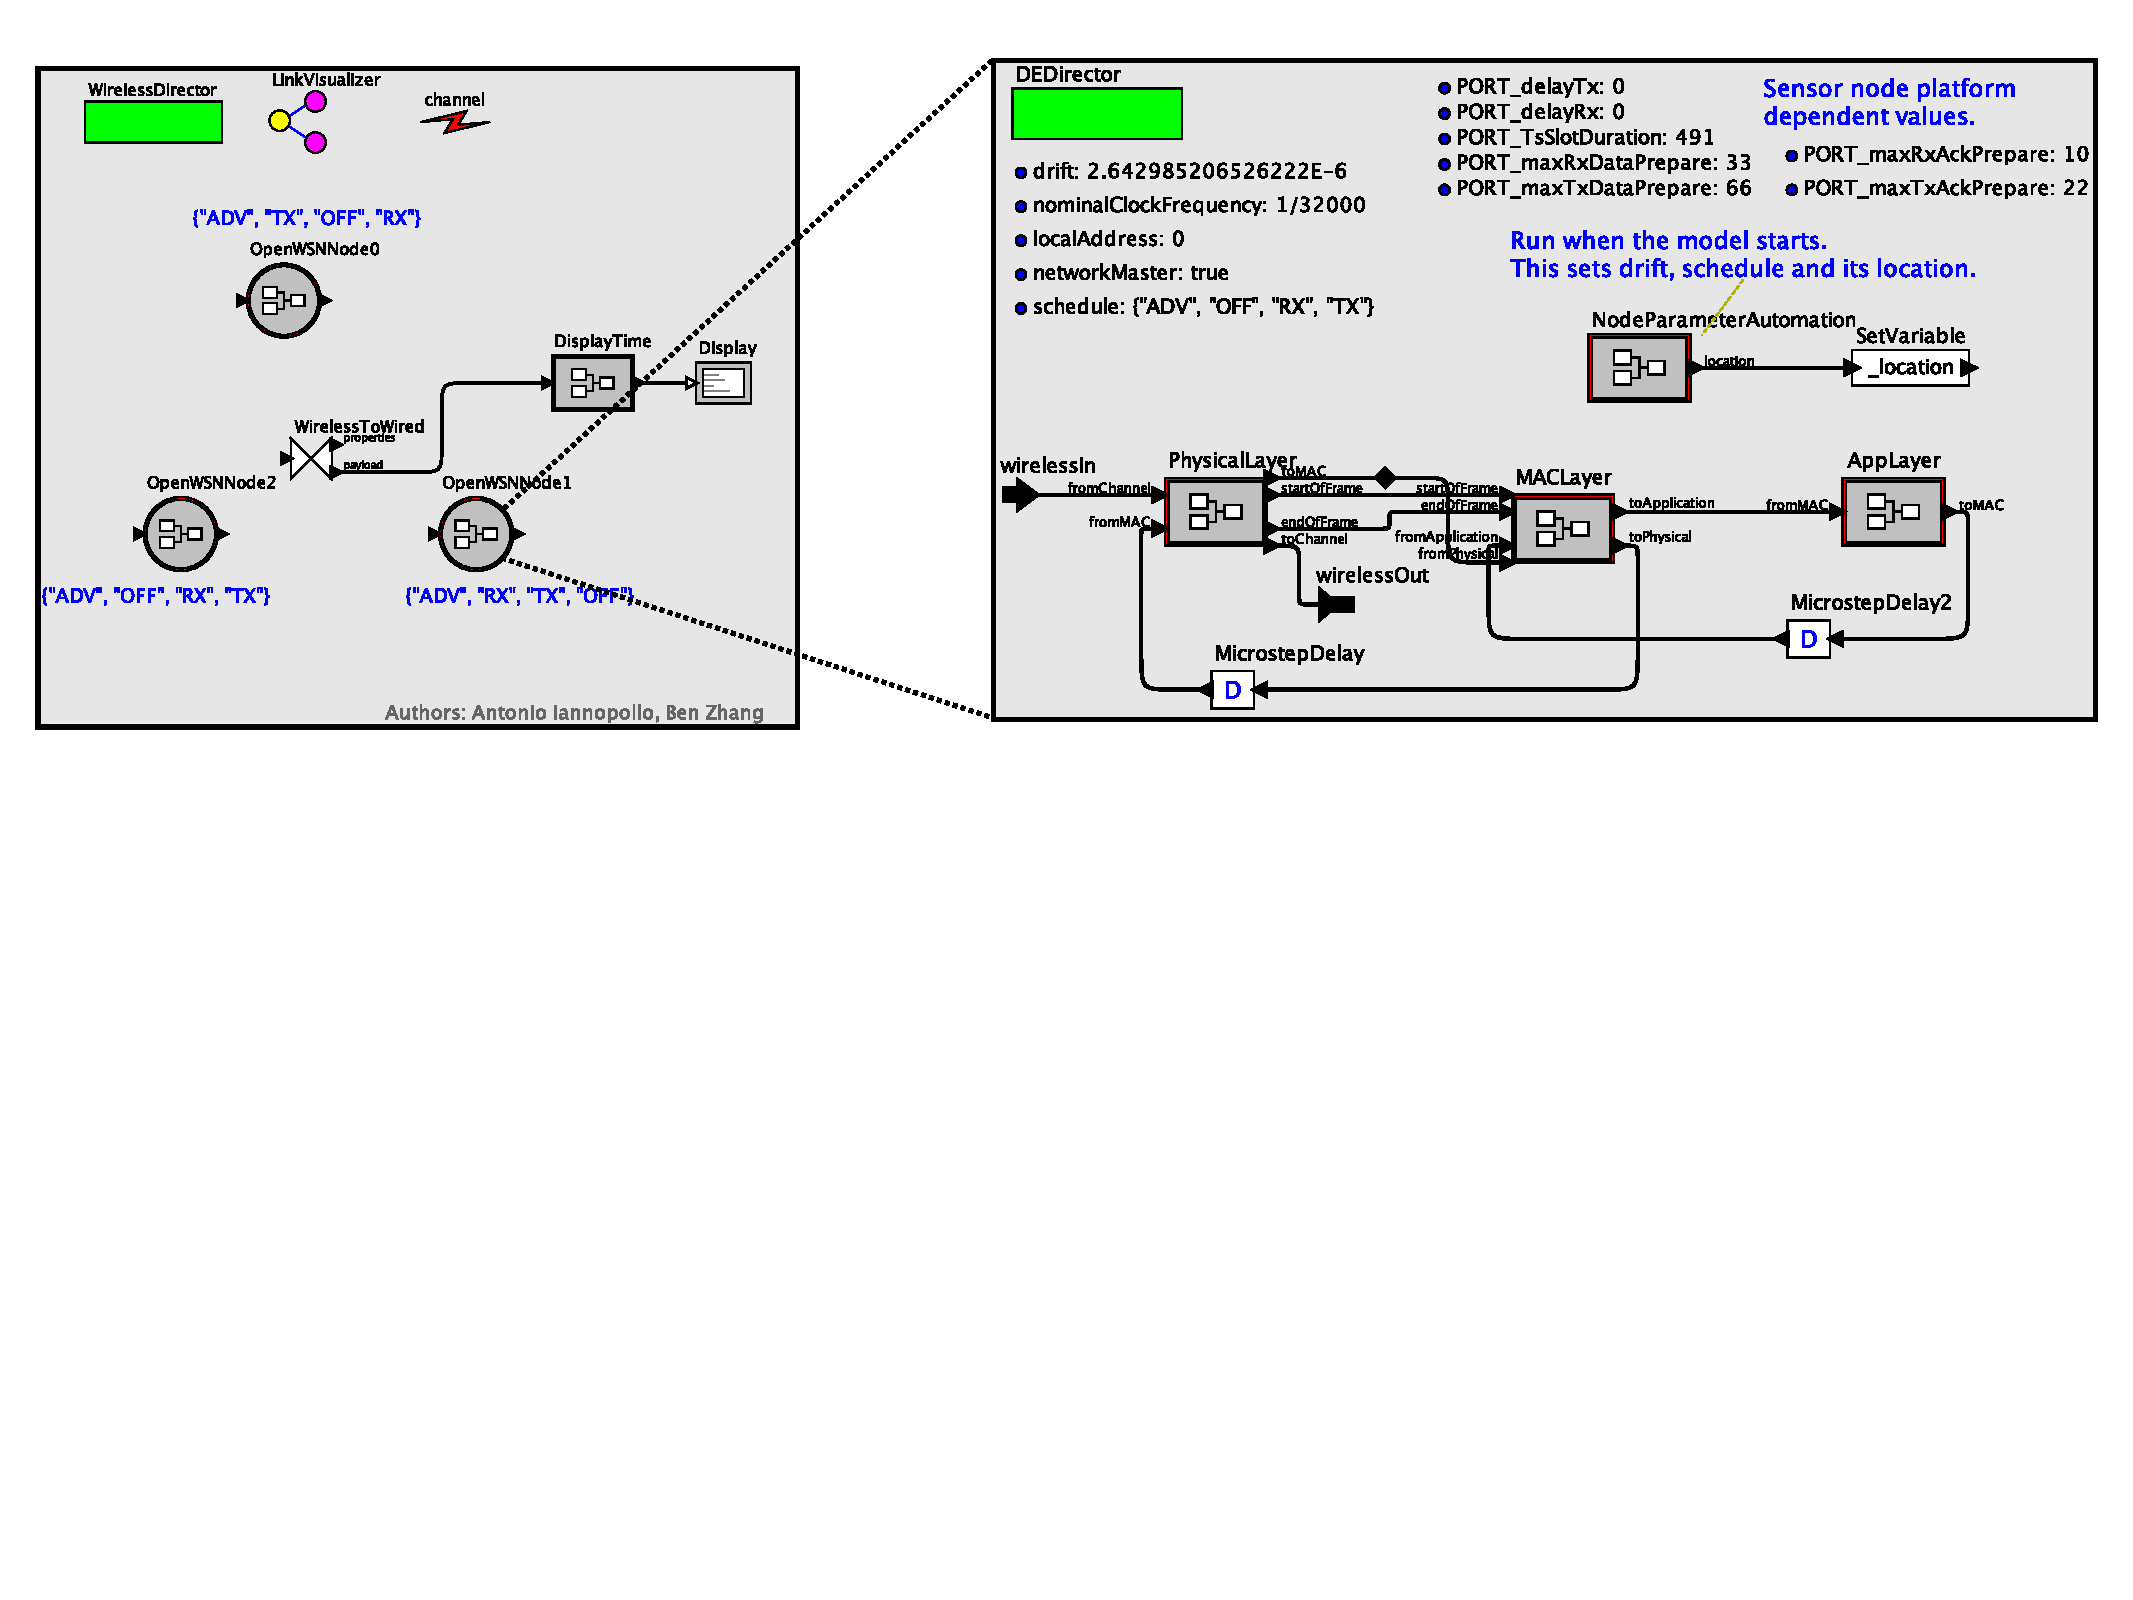
\includegraphics[width=1\columnwidth]{figures/PaperOpenWSNNode}
\caption{An example application of three nodes ({\em left}) and the simplified network stack ({\em right}).}
\label{fig:OpenWSNNode}
\end{figure}

Though our focus is about the TSCH state machine, we have also modeled the physical radio and abstracted the higher layer as application layers (see Figure~\ref{fig:OpenWSNNode}). The interface to Physical layer is mainly achieved with 1) \texttt{startOfFrame} and \texttt{endOfFrame}, which indicate the radio status; 2) \texttt{fromMAC} and \texttt{toMAC}, which conveys the payload. The interface to higher layer (mainly \texttt{AppLayer} in this case) is through \texttt{fromMAC} and \texttt{toMAC} ports. 

Inside the \texttt{MACLayer} actor, we have a few actors including \texttt{packetQueueManager}, \texttt{scheduler}, \texttt{PacketProcessor} and \texttt{TSCHStateMachine}, each does what the name indicates. The major part is the \texttt{TSCHStateMachine}, where we modelled the protocol behavior using Hierarchical Modal Model \ref{fig:TSCHSM}. It consists of five main states \texttt{init}, \texttt{SLEEP}, \texttt{synchronization}, \texttt{tx} and \texttt{rx}. 


\begin{figure}[t]
\centering
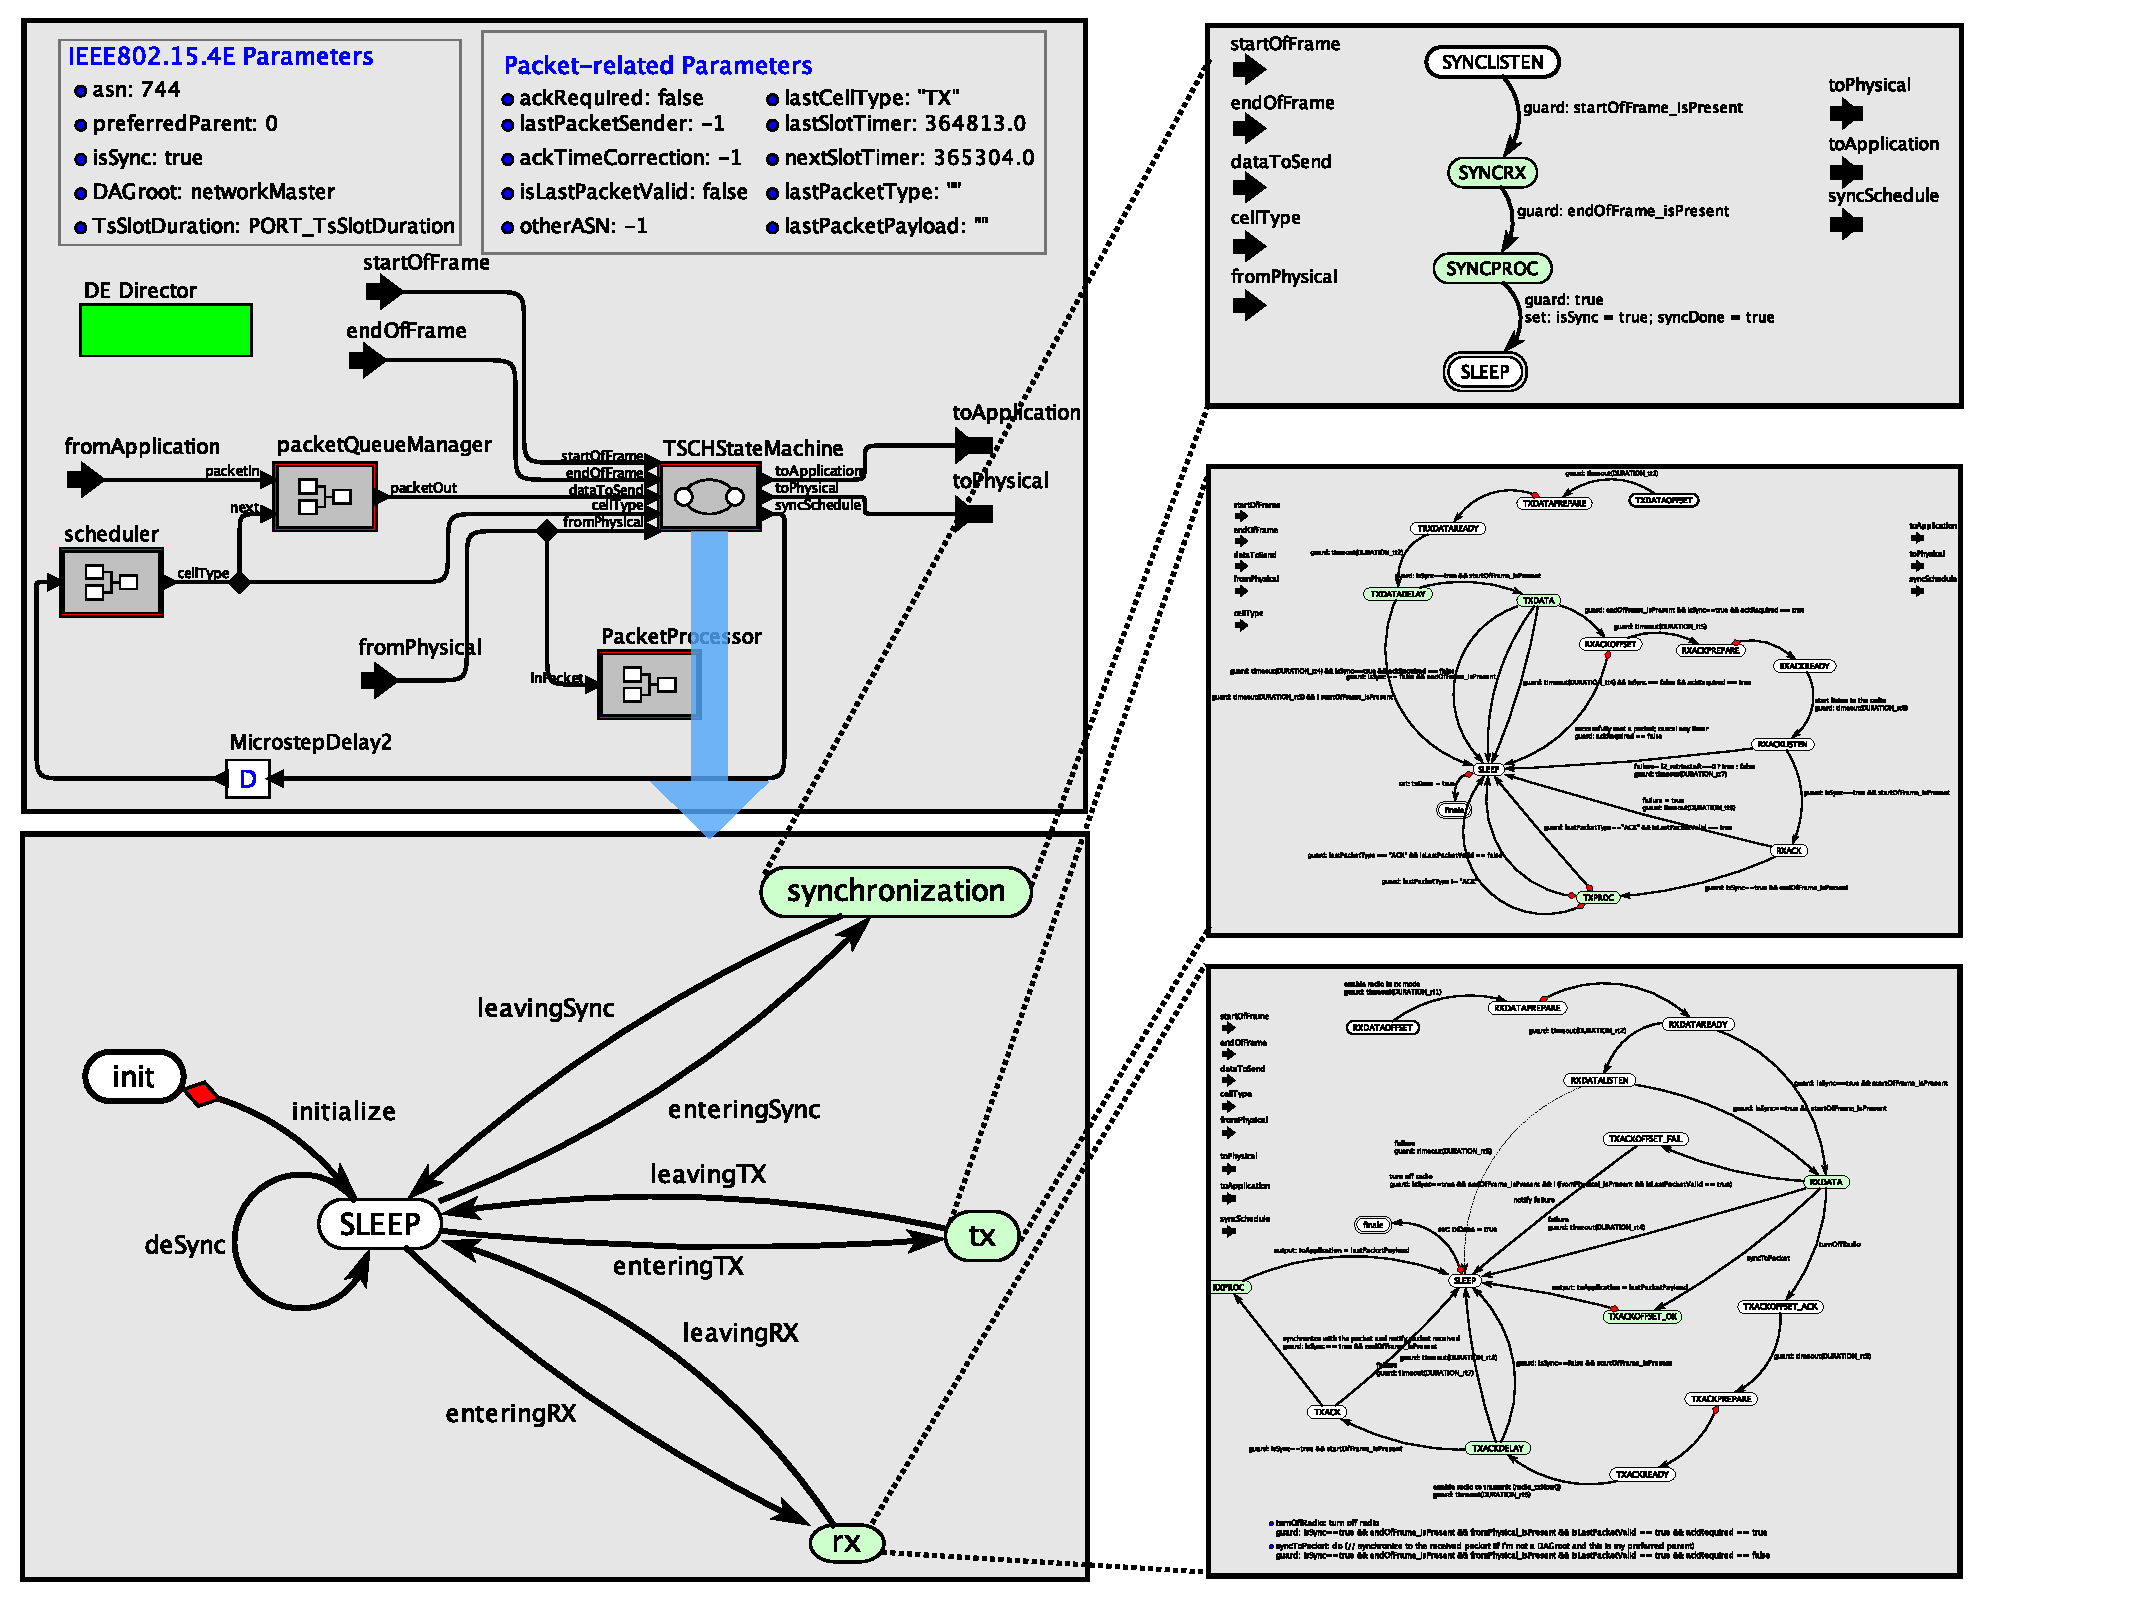
\includegraphics[width=1\columnwidth]{figures/PaperTSCHStateMachine}
\caption{The state machine with refinements of TSCH protocol.}
\label{fig:TSCHSM}
\end{figure}

During initialization, we reset all protocol related parameters, Inside \texttt{synchronization}, the node keeps listening to \texttt{ADV} packet and performs slot synchronization and ASN synchronization. Once the synchronization is done, it goes back to \texttt{SLEEP} state and then its behavior is controlled by the \texttt{scheduler}. 
\begin{itemize}
\item If it's \texttt{ADV} slot, then the node enters \texttt{tx} state and send \texttt{ADV} packet. 
\item If it's \texttt{TX} or \texttt{RXTX} slot and the node has data to send (there are packets queued at \texttt{packetQueueManager}), it will enter \texttt{tx} state too and send the data packet. 
\item If it's \texttt{RX} slot, or it's \texttt{RXTX} slot but the application doesn't have data to send, the node will enter \texttt{rx} state and listen for packets.
\end{itemize}

In \texttt{tx} and \texttt{rx} state, there is the refinement which captures the complicated state transition of the radio. For example, when the node is sending a packet, it first delays a certain time (in \texttt{TXDATAOFFSET} state), then prepares the data for radio to transmit (\texttt{TXDATAPREPARE}), and after a few other states that are used to check the radio status, it finally enters \texttt{TXDATA} state and tranmit the packet. Similar complexity exists for managing ackowledgement and receiving a packet. Given our paper length constrain, we refer the reader to our Ptolemy model for more detail state transition behavior.

The \texttt{synchronization} state above doesn't include resynchronization, which is used to correct the clock drifts among wireless nodes. In fact, for every packet transmission, the receiver will capture the time when it receives the packet (Figure~\ref{fig:timeCorrection} {\em up}). If the packet is from a time master, it will calculate the time discrepancy and use it to determine the next slot boundary (Figure~\ref{fig:timeCorrection} {\em middle}) If the packet is from a time slave, then the node will still perform a calcuation and send the time correction through \texttt{ACK} packet (Figure~\ref{fig:timeCorrection} {\em down}).

\begin{figure}[t]
\centering
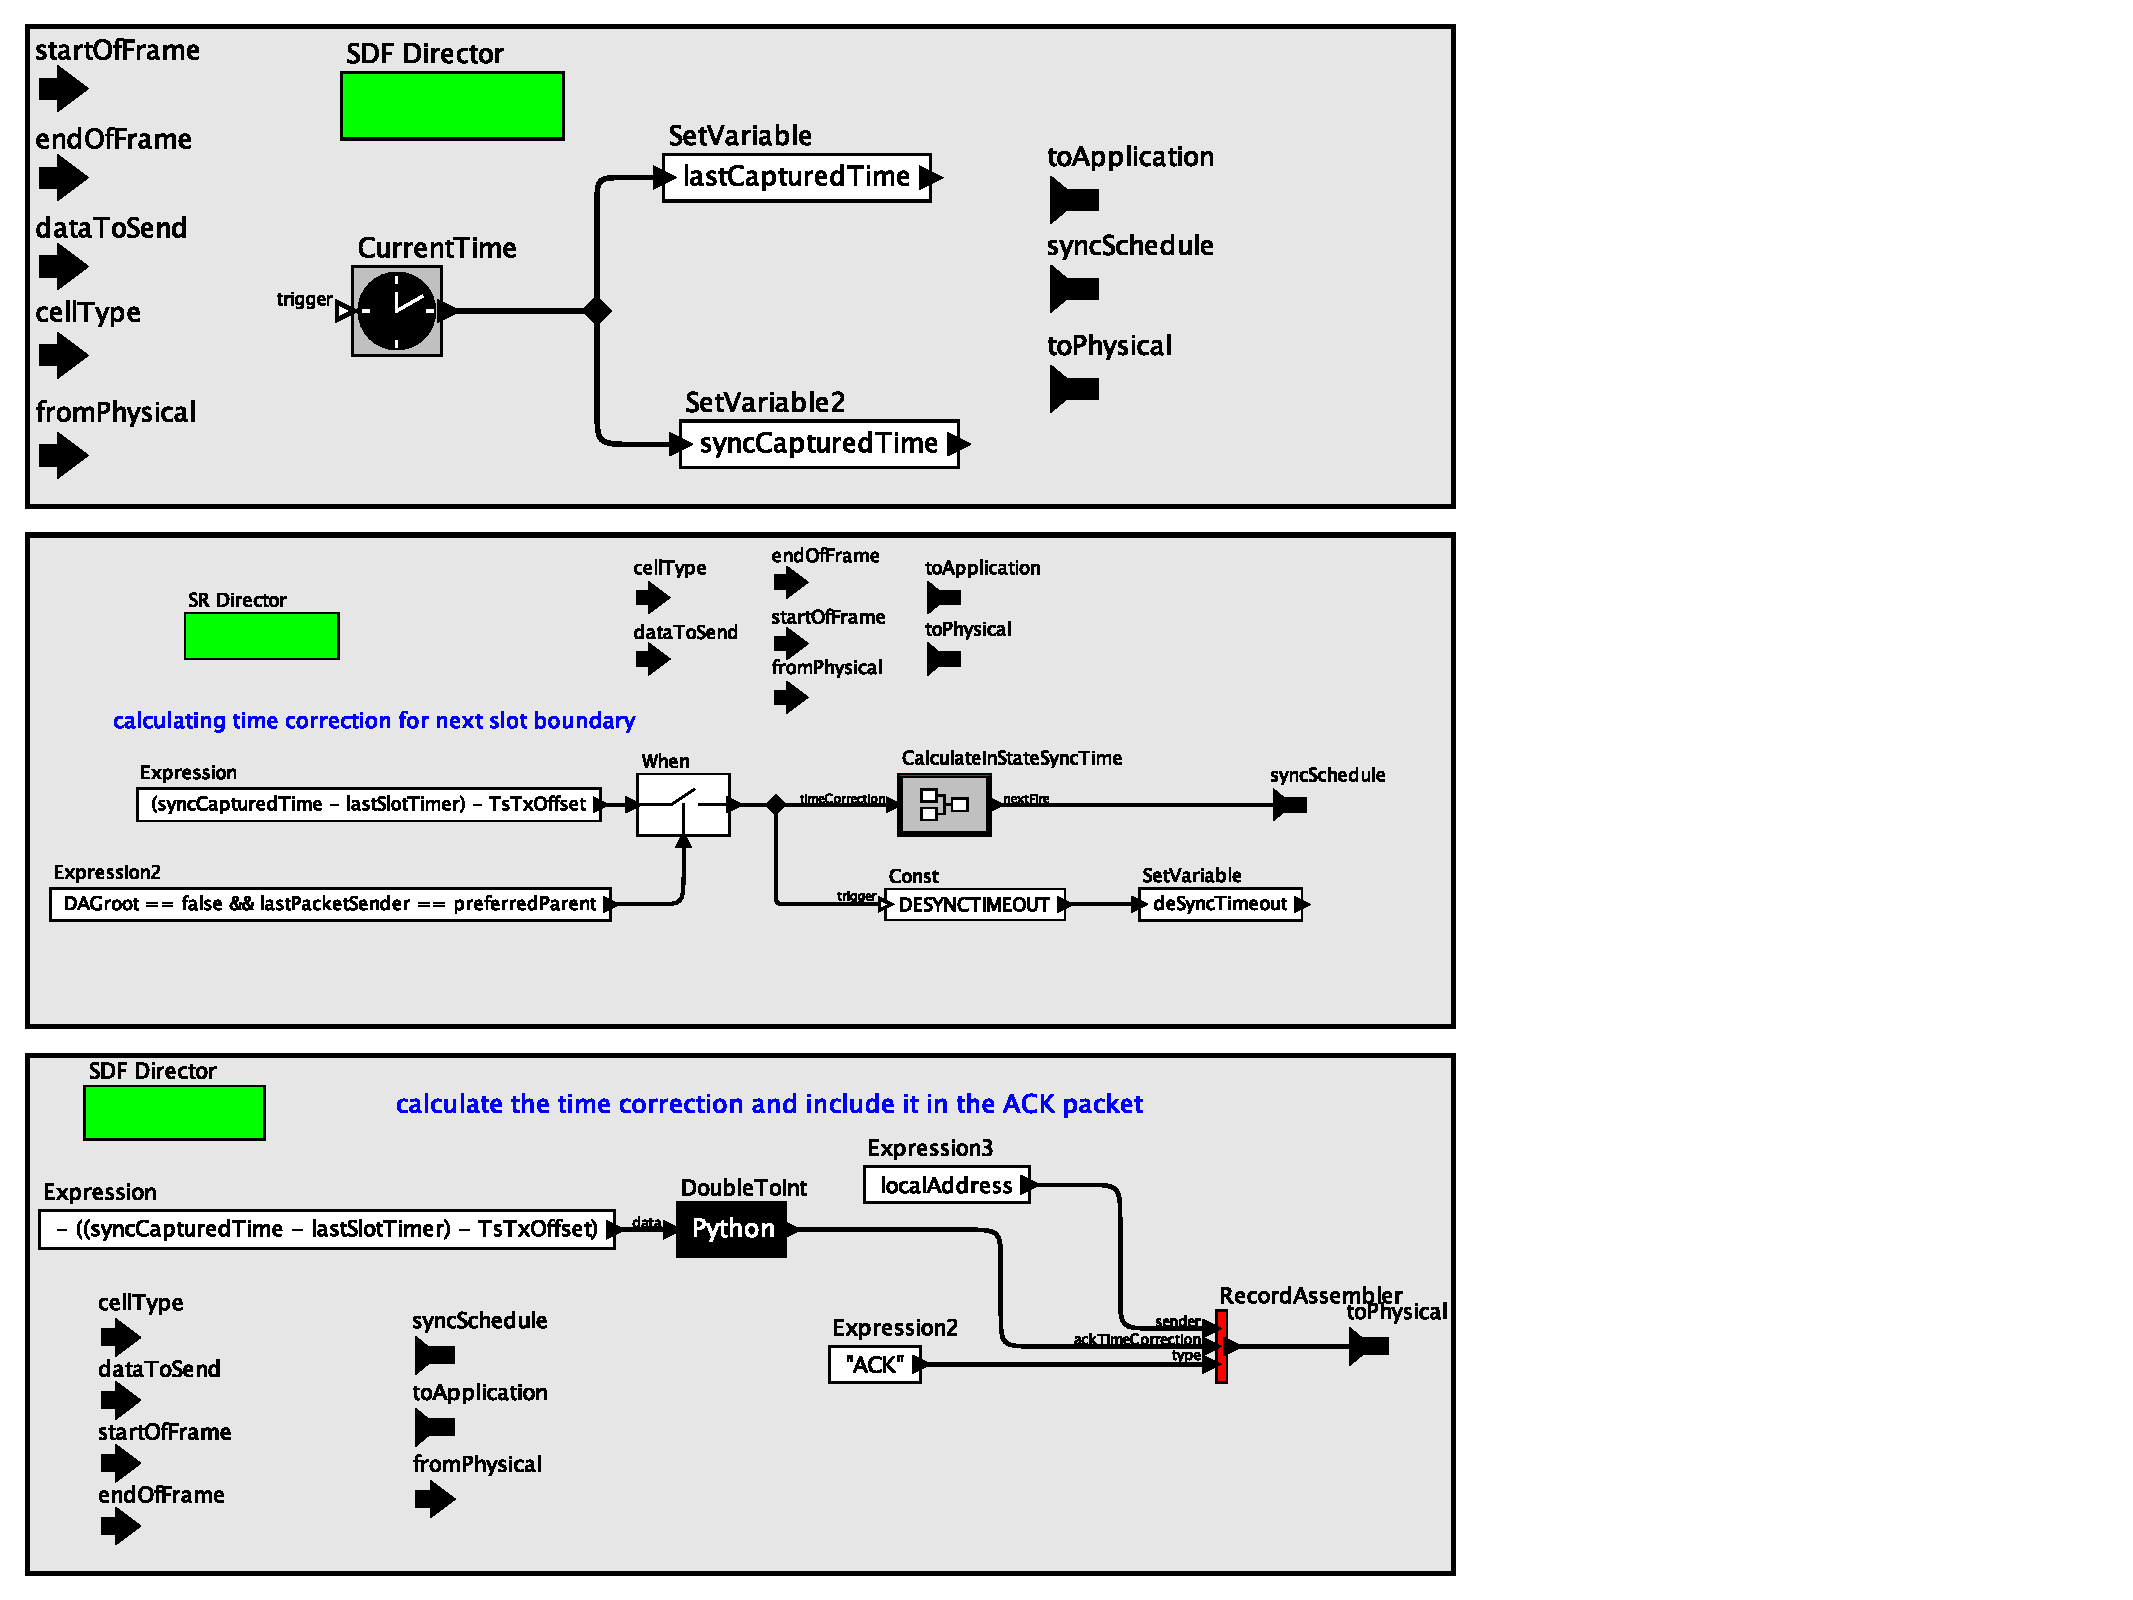
\includegraphics[width=0.9\columnwidth]{figures/PaperReSynchronization}
\caption{Modelling the the resynchronization.}
\label{fig:timeCorrection}
\end{figure}

%%% Local Variables: 
%%% mode: latex
%%% TeX-master: "ee219d"
%%% End: 
